\hypertarget{findNearestPoint_8cpp}{}\section{/home/viki/catkin\+\_\+ws/src/\+Robotic-\/polishing/src/pcl\+\_\+midterm/find\+Nearest\+Point.cpp File Reference}
\label{findNearestPoint_8cpp}\index{/home/viki/catkin\+\_\+ws/src/\+Robotic-\/polishing/src/pcl\+\_\+midterm/find\+Nearest\+Point.\+cpp@{/home/viki/catkin\+\_\+ws/src/\+Robotic-\/polishing/src/pcl\+\_\+midterm/find\+Nearest\+Point.\+cpp}}


This \hyperlink{findNearestPoint_8h_source}{find\+Nearest\+Point.\+h} is a header file of finding the closest point on a post smoothing surface. There are three method in this class. The goal is to get indices array which indicate the closest point with several given points. For example, I can given a arbitrary coordinate and use this class to find a closest point ID from point cloud group.  


{\ttfamily \#include $<$find\+Nearest\+Point.\+h$>$}\\*
{\ttfamily \#include $<$stdlib.\+h$>$}\\*
{\ttfamily \#include $<$pcl/point\+\_\+cloud.\+h$>$}\\*
{\ttfamily \#include $<$pcl/kdtree/kdtree\+\_\+flann.\+h$>$}\\*
{\ttfamily \#include $<$iostream$>$}\\*
{\ttfamily \#include $<$string$>$}\\*
{\ttfamily \#include $<$fstream$>$}\\*
{\ttfamily \#include $<$vector$>$}\\*
{\ttfamily \#include $<$ctime$>$}\\*
Include dependency graph for find\+Nearest\+Point.\+cpp\+:
\nopagebreak
\begin{figure}[H]
\begin{center}
\leavevmode
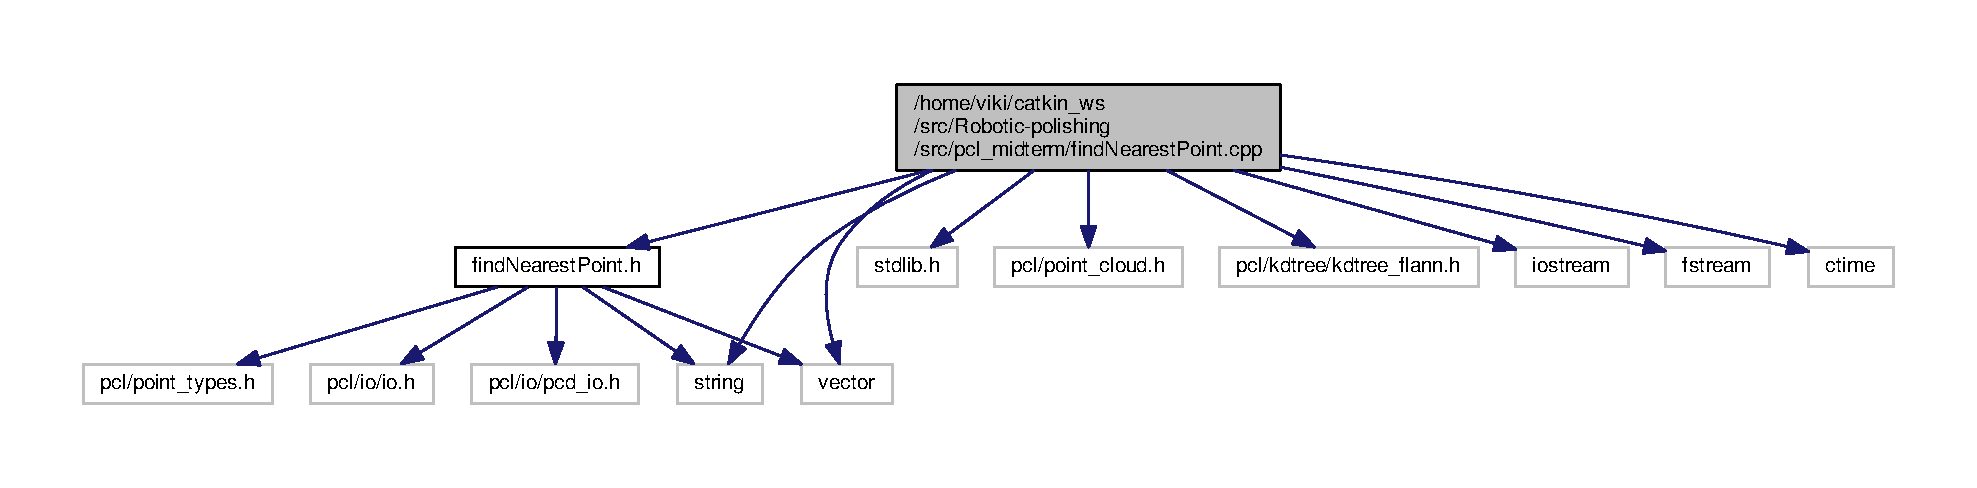
\includegraphics[width=350pt]{findNearestPoint_8cpp__incl}
\end{center}
\end{figure}


\subsection{Detailed Description}
This \hyperlink{findNearestPoint_8h_source}{find\+Nearest\+Point.\+h} is a header file of finding the closest point on a post smoothing surface. There are three method in this class. The goal is to get indices array which indicate the closest point with several given points. For example, I can given a arbitrary coordinate and use this class to find a closest point ID from point cloud group. 

This \hyperlink{findNearestPoint_8cpp}{find\+Nearest\+Point.\+cpp} is an implementation of finding the closest point on a post smoothing surface. There are three method in this class. The goal is to get indices array which indicate the closest point with several given points. For example, I can given a arbitrary coordinate and use this class to find a closest point ID from point cloud group.

\begin{DoxyAuthor}{Author}
Michael Kam (michael081906) 
\end{DoxyAuthor}
\begin{DoxyRefDesc}{Bug}
\item[\hyperlink{bug__bug000005}{Bug}]No known bugs. \end{DoxyRefDesc}
\begin{DoxyCopyright}{Copyright}
G\+NU Public License.
\end{DoxyCopyright}
\hyperlink{classfindNearestPoint}{find\+Nearest\+Point} is free software\+: you can redistribute it and/or modify it under the terms of the G\+NU General Public License as published by the Free Software Foundation, either version 3 of the License, or (at your option) any later version.

\hyperlink{classfindNearestPoint}{find\+Nearest\+Point} is distributed in the hope that it will be useful, but W\+I\+T\+H\+O\+UT A\+NY W\+A\+R\+R\+A\+N\+TY; without even the implied warranty of M\+E\+R\+C\+H\+A\+N\+T\+A\+B\+I\+L\+I\+TY or F\+I\+T\+N\+E\+SS F\+OR A P\+A\+R\+T\+I\+C\+U\+L\+AR P\+U\+R\+P\+O\+SE. See the G\+NU General Public License for more details. You should have received a copy of the G\+NU General Public License along with \hyperlink{classfindNearestPoint}{find\+Nearest\+Point}. If not, see \href{http://www.gnu.org/licenses/}{\tt http\+://www.\+gnu.\+org/licenses/}.

\begin{DoxyAuthor}{Author}
Michael Kam (michael081906) 
\end{DoxyAuthor}
\begin{DoxyRefDesc}{Bug}
\item[\hyperlink{bug__bug000028}{Bug}]No known bugs. \end{DoxyRefDesc}
\begin{DoxyCopyright}{Copyright}
G\+NU Public License.
\end{DoxyCopyright}
\hyperlink{classfindNearestPoint}{find\+Nearest\+Point} is free software\+: you can redistribute it and/or modify it under the terms of the G\+NU General Public License as published by the Free Software Foundation, either version 3 of the License, or (at your option) any later version.

\hyperlink{classfindNearestPoint}{find\+Nearest\+Point} is distributed in the hope that it will be useful, but W\+I\+T\+H\+O\+UT A\+NY W\+A\+R\+R\+A\+N\+TY; without even the implied warranty of M\+E\+R\+C\+H\+A\+N\+T\+A\+B\+I\+L\+I\+TY or F\+I\+T\+N\+E\+SS F\+OR A P\+A\+R\+T\+I\+C\+U\+L\+AR P\+U\+R\+P\+O\+SE. See the G\+NU General Public License for more details. You should have received a copy of the G\+NU General Public License along with \hyperlink{classfindNearestPoint}{find\+Nearest\+Point}. If not, see \href{http://www.gnu.org/licenses/}{\tt http\+://www.\+gnu.\+org/licenses/}. 